%Jennifer Pan, August 2011

\documentclass[10pt,letter]{article}
	% basic article document class
	% use percent signs to make comments to yourself -- they will not show up.

\usepackage{amsmath}
\usepackage{amssymb}
\usepackage{bbm}
	% packages that allow mathematical formatting

\usepackage{graphicx}
	% package that allows you to include graphics

\usepackage{setspace}
	% package that allows you to change spacing

\onehalfspacing
	% text become 1.5 spaced

\usepackage{fullpage}
	% package that specifies normal margins


\begin{document}
	% line of code telling latex that your document is beginning


\title{ECON550: Problem Set 2}

\author{Nicholas Wu}

\date{Fall 2020}
	% Note: when you omit this command, the current dateis automatically included

\maketitle
	% tells latex to follow your header (e.g., title, author) commands.
\section*{HMC Exercises (7th edition)}
\paragraph{1.4.1}
\[ P(C_2 \cup C_3 \cup ... | C_1) = \frac{P(C_1 \cap (C_2 \cup C_3 \cup ...))}{P(C_1)} \]
\[ = \frac{P((C_1 \cap C_2) \cup (C_1 \cap C_3) \cup ...))}{P(C_1)} \]
Since all the $C_2, C_3, ...$ are disjoint,
\[ = \frac{P(C_1 \cap C_2) + P(C_1 \cap C_3) + P(C_1 \cap C_4) + ...}{P(C_1)} \]
\[ = P(C_2 | C_1) + P(C_3 | C_1) + P(C_4 | C_1) + ... \]
\paragraph{1.4.2}
\[ P(C_1 \cap C_2 \cap C_3 \cap C_4) = \frac{P(C_1)}{P(C_1)}\frac{P(C_1 \cap C_2)}{P(C_1 \cap C_2)}\frac{P(C_1 \cap C_2\cap C_3)}{P(C_1 \cap C_2\cap C_3)}P(C_1 \cap C_2 \cap C_3 \cap C_4)\]
\[= P(C_1)\frac{P(C_1 \cap C_2)}{P(C_1)}\frac{P(C_1 \cap C_2\cap C_3)}{P(C_1 \cap C_2)}\frac{P(C_1 \cap C_2 \cap C_3 \cap C_4)}{P(C_1 \cap C_2\cap C_3)}\]
\[= P(C_1) P(C_2 | C_1) P(C_3 | C_1 \cap C_2) P(C_4 | C_1 \cap C_2 \cap C_3) \]
Only using Bayes' rule.
\paragraph{1.4.9}
Let $P(a)$ denote the probability of drawing exactly $a$ blue chips from bowl 1. The probability of drawing a blue chip from the second bowl is then given by
\[ P(0) \frac{0}{5} + P(1) \frac{1}{5} + P(2) \frac{2}{5} + P(3)\frac{3}{5} + P(4)\frac{4}{5} \]
\[ \frac{6}{252}\frac{0}{5} + \frac{60}{252}\frac{1}{5} + \frac{120}{252}\frac{2}{5} + \frac{60}{252}\frac{3}{5} +  \frac{6}{252}\frac{4}{5} \]
The probability of drawing exactly 3 blue chips from bowl I and then drawing a blue chip from bowl II is
\[ \frac{60}{252}\frac{3}{5} \]
Thus, the conditional probability desired is
\[ \frac{180}{60 + 240 + 180 +  24} = \frac{5}{14} \]
\paragraph{1.4.12(c)}
$C_1$ and $C_2^c$ are independent, so
\[ P(C_1 \cap C_2^c) = 0.42 \]
Hence
\[ P(C_1 \cup C_2^c) = P(C_1) + P(C_2^c) - P(C_1 \cap C_2^c) = 0.88 \]
\paragraph{1.4.23}
\[ P(C_1 \cup C_2 \cup C_3) = P(C_1) + P(C_2) + P(C_3) - P(C_1 \cap C_2) - P(C_2 \cap C_3) - P(C_1 \cap C_3) + P(C_1 \cap C_2 \cap C_3) \]
 \[ = \frac{1}{2} + \frac{1}{3} + \frac{1}{4} - \frac{1}{6} - \frac{1}{12} - \frac{1}{8} + \frac{1}{24} = \frac{3}{4} \]
\paragraph{1.5.1}
The induced probability is:
\[ P_X(0) = \frac{9}{13} \]
\[ P_X(1) = \frac{1}{13} \]
\[ P_X(2) = \frac{1}{13} \]
\[ P_X(3) = \frac{1}{13} \]
\[ P_X(4) = \frac{1}{13} \]
\paragraph{1.5.4(c)}
The cdf is given by:
\[ \begin{cases}
      0 & x < 1 \\
      1/15 & 1\leq x< 2 \\
      3/15 & 2 \le x< 3 \\
      6/15 & 3 \le x < 4 \\
      10/15 & 4 \le x < 5 \\
      1 & 5 \le x
   \end{cases}
\]
We have sketched the CDF in red and the PDF in purple in the next page.

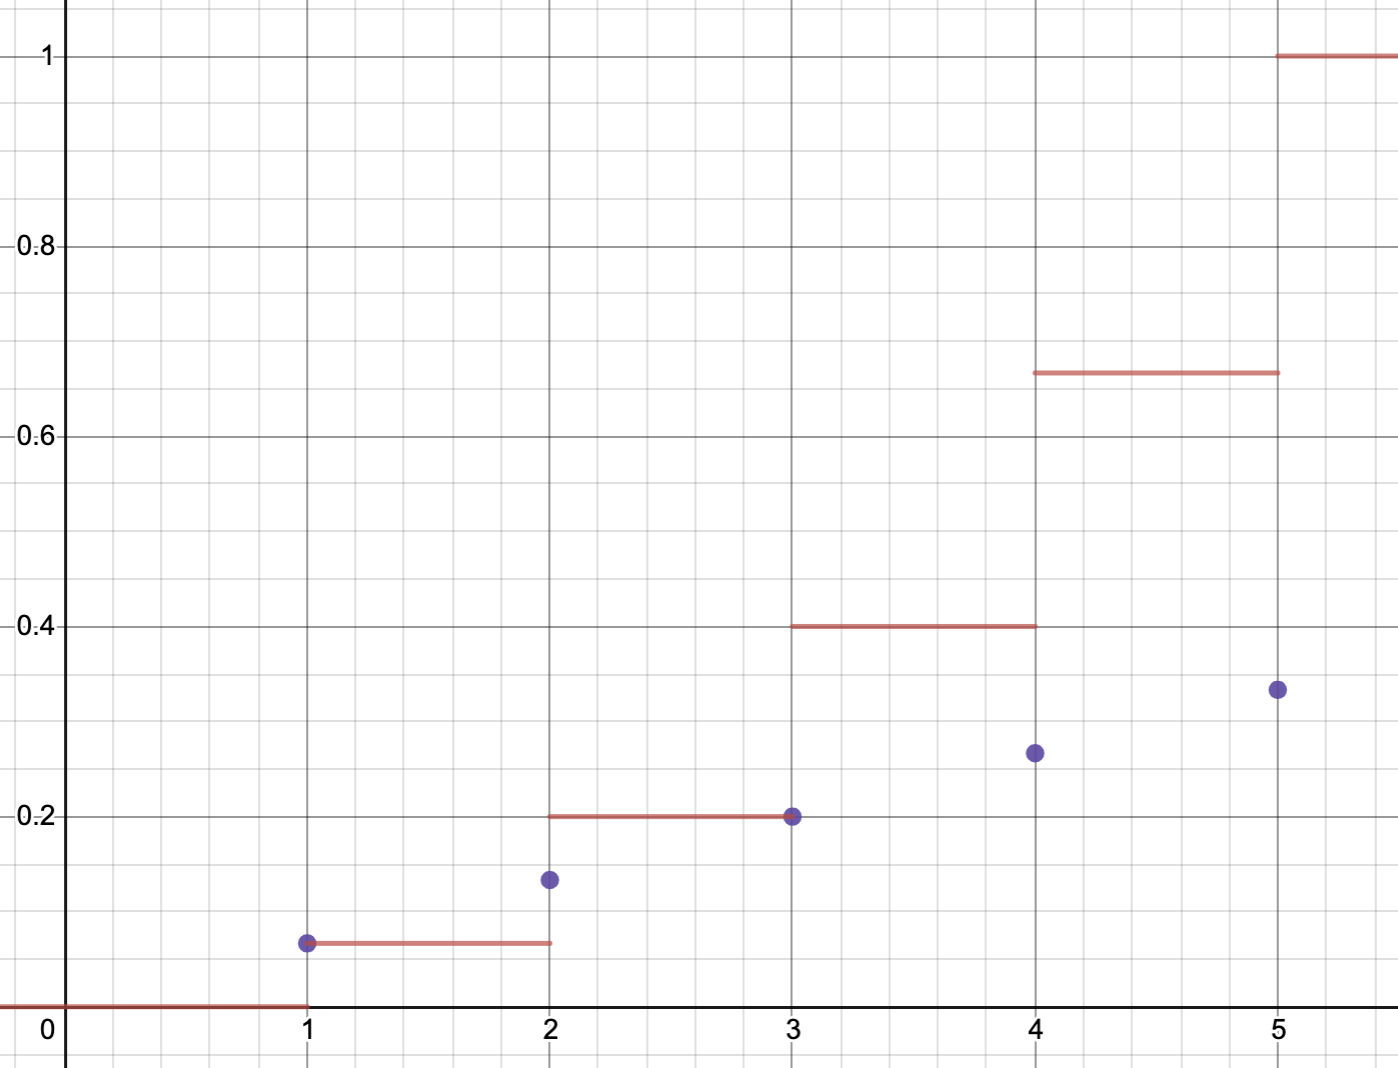
\includegraphics[scale=0.5]{ps2fig1}
\paragraph{1.5.6}
\[ P_X(D_1) = \int_{1}^2 \frac{2x}{9} dx = 1/9 \]
\paragraph{1.5.8(d)} This probability is 0; there is only a nonzero probability for set with a nonempty intersection with $[-1, 1]$.
\paragraph{1.6.3(a)}
The pmf is
\[ p(x) = \frac{1}{6}\left(\frac{5}{6} \right)^{x-1} \]
\paragraph{1.6.3(b)}
\[ \sum p(x) = \sum \frac{1}{6}\left(\frac{5}{6} \right)^{x-1} \]
\[ = \frac{1/6}{1-(5/6)} = 1 \]
\paragraph{1.6.3(d)}
\[ F(x) = \sum_{k=1}^x \frac{1}{6}\left(\frac{5}{6} \right)^{x-1} = 1-\left(\frac{5}{6}\right)^x\]
\paragraph{1.7.1}
CDF:
\[ F_X(x) = \frac{\sqrt{x}}{10} \]
PMF:
\[ f_X(x) = \frac{1}{5\sqrt{x}} \]
\paragraph{1.7.6(a)}
\[ P(|X|<1) = \int_{-1}^1 x^2/18 \ dx = 1/3 \]
\[ P(X^2<9) = 1 \]
\paragraph{1.7.7}
\[ P_X(C_1 \cup C_2) = 1/2 + (1/20) = 11/20 \]
\[ P_X(C_1 \cap C_2) = 0 \]
\paragraph{1.7.9(b)}
Median is
\[ x^3 = \frac{1}{2} \implies x = \frac{1}{\sqrt[3]{2}} \]
\paragraph{1.7.15}
Negating the expression, we get
\[ - P(X > z) \le - P(Y > z) \]
\[ 1 - P(X > z) \le 1 - P(Y > z) \]
\[ P(X \le z) \le P(Y \le z) \]
\[ F_X(z) \le F_Y(z) \]
Strict inequality holding for at least one $z$.
\section*{Problem 4}
We know that
$\lim_{x \to -\infty} F_X(x) = \lim_{x \to -\infty} Pr(X \le x) $
\[ = \lim_{x \to -\infty} 1 - Pr(X > x) \]
\[ = 1 - \lim_{x \to -\infty} Pr(X > x) \]
But as $x \to -\infty$ the interval $(x, \infty) \to \mathbb{R}$, and hence $\lim_{x \to -\infty} Pr(X > x) = Pr(X \in \mathbb{R}) = 1$. Therefore
\[\lim_{x \to -\infty} F_X(x) = 1 - \lim_{x \to -\infty} Pr(X > x) \]
\[ = 1 - 1 = 0 \]
as desired.
\section*{Problem 5}
To show this is a $\sigma$-field, we show this is closed under complements and finite unions. To show closure under complements, consider some $S \in \mathcal{B}(\Omega_X)$. Then we know $\exists B \in \mathcal{B}$ such that
\[ S = B \cap \Omega_X \]

\[ \Omega_X\setminus S = \Omega_X \setminus (B \cap \Omega_X) = \]
\[ = \Omega_X \setminus B = B^c \cap \Omega_X \]
Since $\mathcal{B}$ is a $\sigma$-field, $B^c \in \mathcal{B}$, and hence $S = B^c \cap \Omega_X$ is in $\mathcal{B}(\Omega_X)$.

Now, we show closure under countable union. Consider $S_1, S_2, ... \in \mathcal{B}(\Omega_X)$. We know $\exists B_1, B_2, ... \in \mathcal{B}$ such that $S_i = B_i \cap \Omega_X$. Let
\[S = \cup_i S_i \]
\[ = \cup_i (B_i \cap \Omega_X) \]
\[ = (\cup_i B_i ) \cap (\cup_i \Omega_X) \]
\[ = (\cup_i B_i ) \cap\Omega_X  \]
But $\cup B_i \in \mathcal{B}$ since $\mathcal{B}$ is a $\sigma$-field, and so we have that $S \in \mathcal{B}(\Omega_X)$, and hence we have the closure properties. So $\mathcal{B}(\Omega_X)$ is a $\sigma$-field.

\section*{Problem 6}
Let $s_1, s_2$ be simple functions. Then there exists some disjoint sets $A_j$ such that
\[ s_1(x) = \sum_{j=1}^M c_j 1_{A_j} \]
\[ s_2(x) = \sum_{j=1}^M d_j 1_{A_j} \]
Then
\[ \int (s_1 + s_2) d\mu = \sum_{j=1}^M (c_j + d_j) \mu(A_j) \]
\[ = \sum_{j=1}^M c_j \mu(A_j)+ d_j \mu(A_j)  \]
\[ = \sum_{j=1}^M c_j \mu(A_j)+ \sum_{j=1}^Md_j \mu(A_j)  \]
\[ = \int s_1 d\mu + \int s_2 d\mu \]
Further, we have that
\[ \int as_1 d\mu = \sum_{j=1}^M ac_j \mu(A_j) \]
\[ = a \sum_{j=1}^M c_j \mu(A_j) \]
\[ = a \int s_1 d\mu \]
So we have linearity of the Lesbesgue integral on simple functions.
\section*{Problem 7}
We first show linearity for nonnegative, measureable functions. Suppose we have two such functions $f$, $g$. Then, we note that we can construct two increasing sequences of simple functions $\{ s_n \} \to f, \{ s'_n \} \to g$, such that by the monotone convergence
\[ \int f d\mu = \lim_{n \to \infty} \int s_n d\mu \]
\[ \int g d\mu = \lim_{n \to \infty} \int s'_n d\mu \]
So
\[ \int f d\mu + \int g d\mu = \lim_{n \to \infty}\left( \int s_n d\mu + \int s'_n d\mu \right) \]
By linearity of simple functions as we showed in the previous problem,
\[ \int f d\mu + \int g d\mu = \lim_{n \to \infty}\left( \int s_n d\mu + \int s'_n d\mu \right) \]
\[ = \lim_{n \to \infty}\left( \int (s_n + s'_n) d\mu \right) \]
We note then that the sequence $s^*_n = s_n + s'_n$ must also be increasing, since both $s_n$ and $s'_n$ are increaasing. Further, $\{ s^*_n \} \to f+g$.
Hence
\[ \int f d\mu + \int g d\mu = \lim_{n \to \infty}\left( \int (s_n + s'_n) d\mu \right) \]
\[ = \int (f + g) d\mu \]
We also know that for scalar $a$, $\{ as_n \} \to af$, and hence
\[ \int af d \mu =  \lim_{n \to \infty} \int a s_n d\mu\]
\[  =  \lim_{n \to \infty} a \int s_n d\mu\]
\[ = a \lim_{n \to \infty} \int s_n d\mu \]
\[ = a \int f d\mu \]
So Lebesgue integration is linear for nonnegative, measureable functions.

Now more generally, suppose $f$, $g$ are integrable. Then we have
for $f = f^+ - f^-$, $g = g^+ - g^-$. $f^+$, $g^+$, $f^-$, $g^-$ all nonnegative. Then
\[ \int f d \mu = \int f^+ d\mu - \int f^- d\mu \]
\[ \int g d \mu = \int g^+ d\mu - \int g^- d\mu \]
\[ \int f d \mu + \int g d \mu =  \int f^+ d\mu - \int f^- d\mu + \int g^+ d\mu - \int g^- d\mu\]
\[ = \int (f^+ + g^+) d\mu - \int (f^- + g^-) d\mu  \]
\[ = \int ((f^+ + g^+)  - (f^- + g^-)) d\mu  \]
\[ = \int (f + g) d\mu \]
using the linearity of nonnegative functions we proved earlier. Further,
\[ \int af d\mu = \int af^+ d\mu - \int af^- d\mu \]
\[ = a \left(\int f^+ d\mu - \int f^- d\mu \right) \]
\[ = a \int f d\mu \]
So we have shown linearity of the Lebesgue integral on integrable functions.
\end{document}
	% line of code telling latex that your document is ending. If you leave this out, you'll get an error
